\documentclass[11pt]{article}
\usepackage[utf8]{inputenc}
\usepackage{times}
\usepackage{graphicx}
\usepackage{subfigure}

\title{
\includegraphics[scale=1]{fs}}
\author{Paweł Łupkowski\\pawel.lupkowski@gmail.com}
\date{\today}



\begin{document}
\maketitle


\section*{Introduction}

\noindent
The \textit{Fancyslides} class is prepared for short presentations with modern look \& feel. It offers the following features:
\begin{itemize}
\item custom background for each slide,
\item predefined types of slides,
\item simplified commands (e.g. for starting and ending slide).
\end{itemize}

The class is build upon \LaTeX{} Beamer, so all the commands you know should work.  


\section*{Compilation}

\noindent
Presentations prepared in \textit{Fancyslides} should be compiled with \textbf{pdflatex}\\ (see example.tex).


\section*{Author, title and stuff}

To add author, title, affiliation and email information use the following commands from the preamble:

\begin{verbatim}
\newcommand{\titlephrase}{MAKE YOUR POINT CLEAR...}
\newcommand{\name}{Your Name}
\newcommand{\affil}{Organisation}
\newcommand{\email}{your.email@domain.com}
\end{verbatim}


To generate the title slide use the command {\tt \textbackslash startingslide} after the begin document command. There is no need to put the {\tt \textbackslash startingslide} command inside the {\tt frame} environment. Title slide looks like the one presented in Figure \ref{fig:1}.


\section*{Slides}

A slide structure is the following:

\begin{verbatim}
\fbckg{1}
\begin{frame}
\pointedsl{your point}
\end{frame}
\end{verbatim}

So, to generate slide you use standard Beamer's \texttt{frame} environment. Before the opening command you should put {\tt \textbackslash fbckg\{ \}} command. As an argument you put the name of a picture to set as a background image for the slide.

Inside the \texttt{frame} environment you may put the following predefined commands (see Figure \ref{fig:2}):
\begin{itemize}
\item {\tt \textbackslash pointedsl\{your point\}} -- to generate slide with a point with a text inside (only one line of text is allowed here);
\item \texttt{\textbackslash framedsl\{explained clearly\}} -- to generate a slide with a frame with a text inside (linebreaks are possible)
\item {\tt \textbackslash itemized\{\textbackslash item BEAMER EASE OF USE \textbackslash item STH \textbackslash item STH ELSE\}} -- slide with a frame and itemize environment inside. To introduce new item simply use {\tt \textbackslash item} command. There is no need to open and close the itemize environment;
\item {\tt \textbackslash misc\{\ anything you want \}} -- slide with a frame to put anything you like inside it (e.g. a barchart or a picture, quotation etc.).
\item {\tt \textbackslash sources\{\ list of resources \}} -- slide with a~frame and `SOURCES' note, designed to provide information about sources of graphics or fonts used.
\end{itemize}


\begin{figure}
  \centering
\mbox{\subfigure[pointedsl]{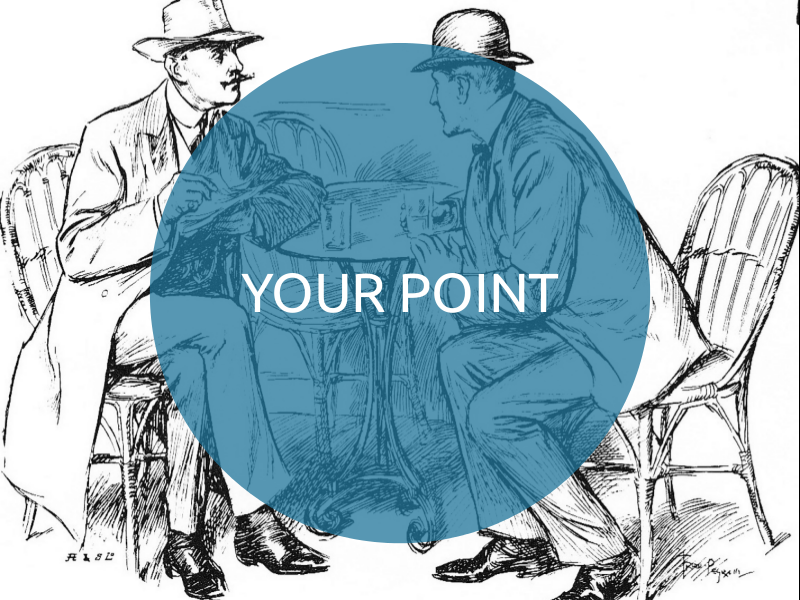
\includegraphics[scale=0.12]{point}} \quad
\subfigure[framedsl]{
\includegraphics[scale=0.12]{frame}} \quad
\subfigure[itemized]{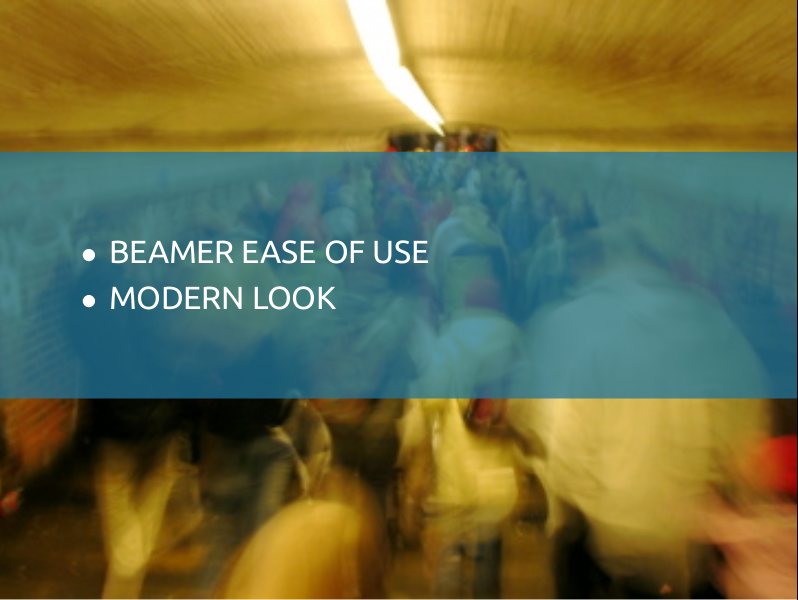
\includegraphics[scale=0.12]{item}} }
  \caption{Three predefined slide types}
  \label{fig:2}
\end{figure}

\noindent
If you want to \textbf{uncover} your content \textbf{step by step} you can use the {\tt \textbackslash pitem} command inside {\tt framedsl}. Simply put your point as an argument of {\tt pitem}. {\tt pitem} will generate an item with {\tt pause} at the end. The last item should be introduced by the {\tt fitem} command (no {\tt pause} after this command is used).

\begin{verbatim}
\fbckg{7}
\begin{frame}
\framedsl{\pitem{pointed slogan} \pitem{framed slogan} 
\pitem{beamer features} \fitem{fonts with xelatex}}
\end{frame}
\end{verbatim}


To generate the {\bf end slide} with thank you note simply use {\tt \textbackslash thankyou} command inside the \texttt{frame} environment. (This will generate \texttt{pointedsl} with THANK YOU note inside.)
\begin{verbatim}
\fbckg{your background}
\begin{frame}
  \thankyou   
\end{frame}
\end{verbatim}




\section*{Structure  elements: opacity and colour}

To change the opacity for the structure elements (boxes and dots) change the value in
\begin{verbatim}
\newcommand{\structureopacity}{0.75}
\end{verbatim}


To change the colour of the structure elements use the following command:
\begin{verbatim}
\newcommand{\strcolor}{orange}
\end{verbatim}
Three colours are predefined (see Figure \ref{fig:1}):
\begin{itemize}
\item blue
\item green
\item orange
\end{itemize}

\begin{figure}
  \centering
\mbox{\subfigure[blue]{
\includegraphics[scale=0.12]{blue}} \quad
\subfigure[green]{
\includegraphics[scale=0.12]{green}} \quad
\subfigure[orange]{
\includegraphics[scale=0.12]{orange}} }
  \caption{Three predefined colours for structure elements}
  \label{fig:1}
\end{figure}

\noindent
To change a text colour use the command 
\begin{verbatim}
\newcommand{\yourowntexcol}{colour name}
\end{verbatim}
where you can put your desired colour name as an argument. 

You can also define your own colour (using RGB values) and use it in this command.\footnote{Easiest way to do this is to use the Inkscape. Simply draw a rectangle and pick up a colour you would like to use. Then choose \textit{Save as...} and point \textit{\LaTeX\ with Pstricks}. Afterwards you may open the result *.tex file and copy the colour definition from it.}




\section*{Fancyslides package}
The \textit{Fancyslides} package contains:
\begin{itemize}
\item \textit{fancyslides.cls} -- document class;
\item \textit{example.tex} -- an exemplary file ready to compile it with \textit{pdflatex};
\item \textit{example.pdf} -- a compiled example, to give you an impression of the \textit{Fancsyslides} look \& feel;
\item \textit{blank.jpg}, \textit{1.jpg} and \textit{2.jpg} -- exemplary background graphics;
\item \textit{fancyslides.pdf} -- this short intro.
\end{itemize}



\section*{Acknowledgments}
I would like my thanks to B.~Marciniak, K.~Paluszkiewicz, M.~Urbański, I.~Furió and S.~Wawrykiewicz for testing, helpful comments and remarks.




\end{document}
